
\cleardoublepage
\appendix
% --- Start Anhang (A, B, C, ...) ---
\setcounter{chapter}{0} % 1 -> A
\renewcommand{\thechapter}{\Alph{chapter}}
\renewcommand{\thesection}{\thechapter.\arabic{section}}
\renewcommand{\thesubsection}{\thesection.\arabic{subsection}}
\renewcommand{\thesubsubsection}{\thesubsection.\arabic{subsubsection}}

% --- Hyperref: eindeutige Link-Anker (wichtig für korrektes Inhaltsverzeichnis) ---
\renewcommand{\theHchapter}{app.\Alph{chapter}}
\renewcommand{\theHsection}{\theHchapter.\arabic{section}}
\renewcommand{\theHsubsection}{\theHsection.\arabic{subsection}}
\renewcommand{\theHsubsubsection}{\theHsubsection.\arabic{subsubsection}}
% =====================================================
% Anhang A: Mathematische Herleitungen
% =====================================================
\chapter{Mathematische Herleitungen}
\label{app:mathematische-herleitungen}

In diesem Anhang werden die im Haupttext angesprochenen physikalischen Konzepte
formal und mathematisch vertieft. Ziel ist es, die didaktische Lesbarkeit der
Kapitel nicht zu beeinträchtigen und zugleich interessierten Leserinnen und Lesern
die wichtigsten Herleitungen zugänglich zu machen.

Die Abschnitte sind thematisch nach zentralen Eigenschaften und Experimenten des
Elektrons\index{Elektron} gegliedert. Dazu gehören unter anderem das
Ladung-Masse-Verhältnis\index{Ladung-Masse-Verhältnis}, die Bestimmung der
Elementarladung\index{Elementarladung}, die Bewegung geladener Teilchen in
elektrischen und magnetischen Feldern\index{elektrisches Feld}\index{Magnetfeld},
sowie quantenmechanische Eigenschaften wie Spin\index{Spin}, Wellenfunktion\index{Wellenfunktion}
und Aufenthaltswahrscheinlichkeit\index{Aufenthaltswahrscheinlichkeit}.

Auf diese Weise bildet der Anhang eine Brücke zwischen den anschaulichen Erklärungen
im Haupttext und der mathematischen Beschreibung des Elektrons in klassischer Physik,
Quantenmechanik\index{Quantenmechanik}, Relativitätstheorie\index{Relativitätstheorie}
und moderner Teilchenphysik\index{Teilchenphysik}.



%\section{Kapitel I}
\phantomsection
% =====================================================
% Bestimmung des Ladung-Masse-Verhältnisses nach Thomson
% =====================================================
\section{Bestimmung des Ladung-Masse-Ver-\newline hältnisses nach Thomson}
\label{app:thomson-qm-herleitung}

J. J. Thomson\index{Thomson, J. J.} bestimmte im Jahr 1897 nicht direkt die
Masse des Elektrons und auch nicht dessen einzelne elektrische Ladung. Beides war
damals noch unbekannt. Er untersuchte vielmehr Kathodenstrahlen\index{Kathodenstrahl}
und zeigte, dass sie sich wie Ströme negativ geladener Teilchen verhalten.

Historisch sauber formuliert ging Thomson also von Teilchen mit unbekannter Ladung
\(q\) und unbekannter Masse \(m\) aus. Sein Ziel war es, aus der Ablenkung dieser
Teilchen in elektrischen und magnetischen Feldern das Verhältnis
\[
\frac{q}{m}
\]
zu bestimmen. Dieses Verhältnis nennt man das Ladung-Masse-Verhältnis
\index{Ladung-Masse-Verhältnis}.

\subsection*{Elektrische Ablenkung}

Ein Teilchen mit der Ladung \(q\) erfährt in einem elektrischen Feld
\index{elektrisches Feld} der Feldstärke \(E\) die Kraft
\[
F_\mathrm{el} = qE.
\]
Nach dem zweiten Newtonschen Gesetz gilt
\[
F = ma.
\]
Setzt man beide Ausdrücke gleich, erhält man
\[
ma = qE.
\]
Damit folgt für die Beschleunigung:
\[
a = \frac{qE}{m}.
\]

Diese Gleichung zeigt bereits den entscheidenden Punkt: Die Ablenkung eines geladenen
Teilchens hängt nicht nur vom elektrischen Feld ab, sondern vom Verhältnis seiner
Ladung zu seiner Masse.

Da Thomson zunächst nicht wusste, wie groß \(q\) und \(m\) einzeln sind, war gerade
das Verhältnis
\[
\frac{q}{m}
\]
die experimentell zugängliche Größe.

\begin{MathBox}[Warum Thomson das Verhältnis \(q/m\) bestimmte]
	\label{box:thomson-qm-statt-einzelwerte}
	Thomson kannte weder die Ladung noch die Masse der Kathodenstrahlteilchen einzeln.
	Aus der Ablenkung im elektrischen Feld ergab sich aber eine Größe, die beide
	miteinander verbindet:
	\[
	a = \frac{qE}{m}.
	\]
	
	Damit war nicht \(q\) allein und auch nicht \(m\) allein messbar, sondern zunächst
	das Verhältnis
	\[
	\frac{q}{m}.
	\]
\end{MathBox}

\subsection*{Magnetische Ablenkung}

Bewegt sich ein geladenes Teilchen mit der Geschwindigkeit \(v\) senkrecht zu einem
Magnetfeld\index{Magnetfeld} der Flussdichte \(B\), so erfährt es die magnetische
Lorentzkraft\index{Lorentzkraft}
\[
F_\mathrm{mag} = qvB.
\]

Diese Kraft wirkt senkrecht zur Bewegungsrichtung. Sie ändert daher vor allem die
Richtung der Bewegung und kann den Kathodenstrahl ablenken.

Thomson nutzte elektrische und magnetische Felder, um das Verhalten der
Kathodenstrahlen gezielt zu untersuchen. Besonders wichtig war der Fall, in dem sich
elektrische und magnetische Ablenkung gegenseitig aufhoben. Dann lief der Strahl
geradlinig weiter.

In diesem Fall gilt dem Betrag nach:
\[
|F_\mathrm{el}| = |F_\mathrm{mag}|.
\]
Also:
\[
|q|E = |q|vB.
\]
Die unbekannte Ladung \(|q|\) kürzt sich heraus:
\[
E = vB.
\]
Damit erhält man die Geschwindigkeit der Teilchen:
\[
v = \frac{E}{B}.
\]

Das ist ein wichtiger Schritt: Die Geschwindigkeit der Kathodenstrahlteilchen lässt
sich bestimmen, ohne die einzelne Ladung oder die Masse des Teilchens bereits zu
kennen.

\begin{MathBox}[Bestimmung der Geschwindigkeit]
	\label{box:thomson-geschwindigkeit-qm}
	Wenn elektrische und magnetische Ablenkung einander gerade aufheben, gilt:
	\[
	|q|E = |q|vB.
	\]
	
	Die unbekannte Ladung kürzt sich heraus. Dadurch folgt:
	\[
	v = \frac{E}{B}.
	\]
	
	Die Geschwindigkeit der Teilchen kann also aus den bekannten Feldgrößen bestimmt
	werden.
\end{MathBox}
\newpage
\noindent
\subsection*{Ablenkung im elektrischen Feld}
Abbildung~\ref{fig:thomson-ablenkung-y1-y2} zeigt die geometrische Zerlegung der
Gesamtablenkung. Sie macht deutlich, warum die beobachtete Ablenkung auf dem Schirm
aus zwei Anteilen besteht.
\FloatBarrier

\begin{figure}[H]
	\centering
	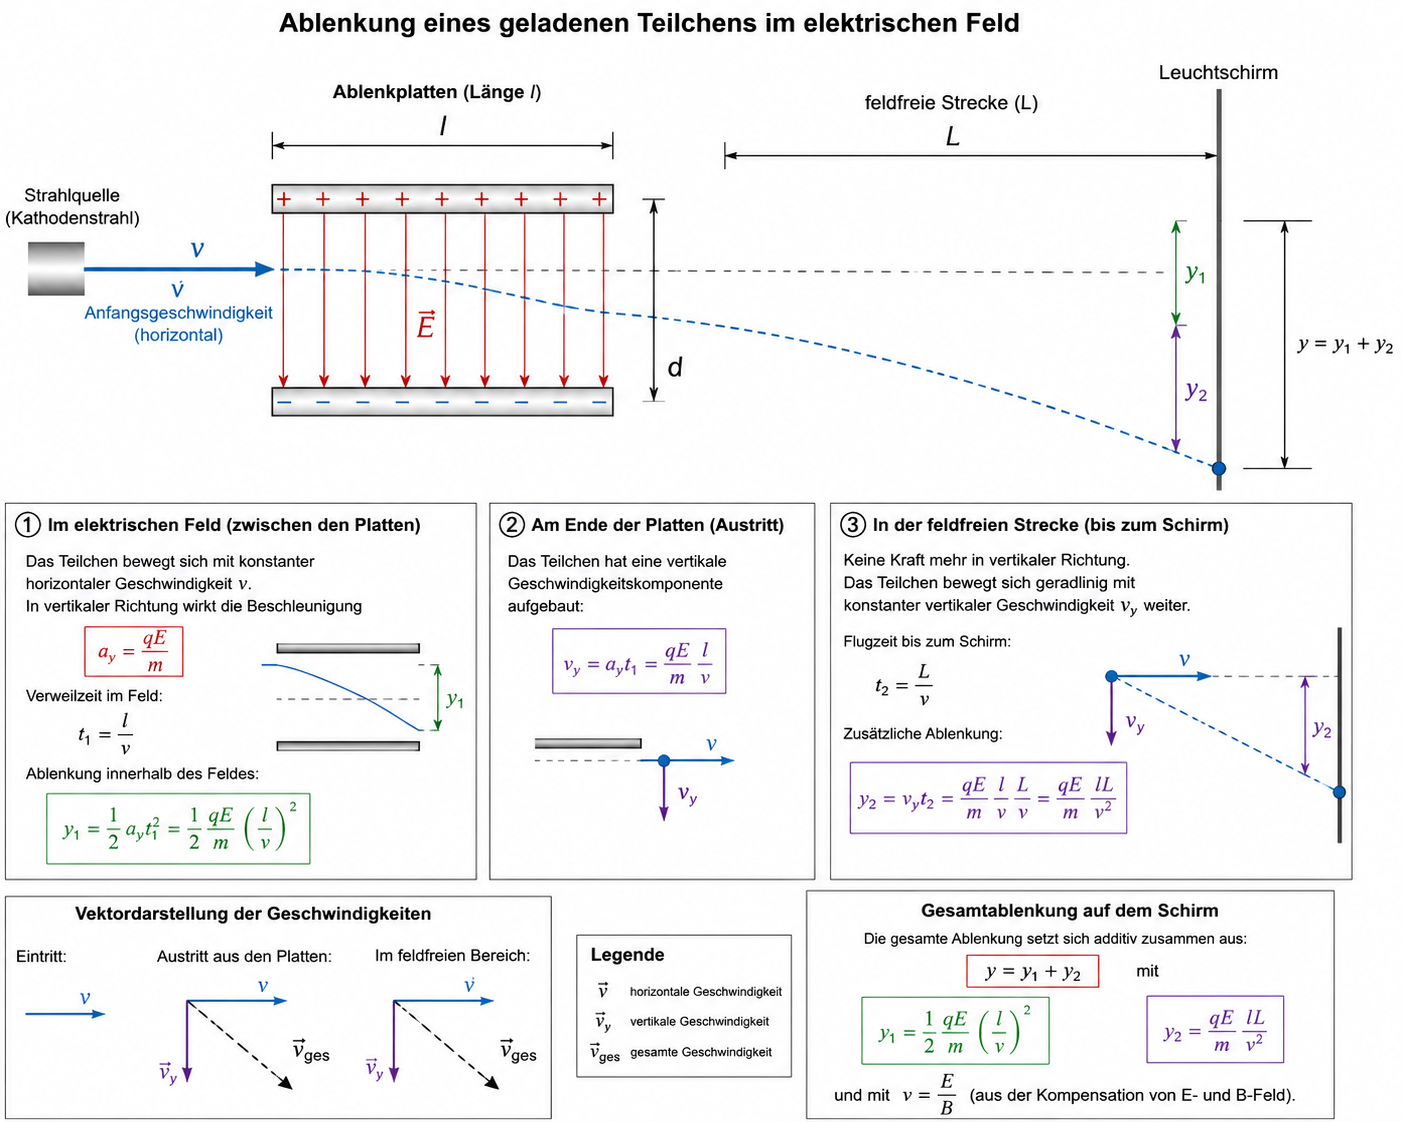
\includegraphics[width=\textwidth]{bilder/thomson_ablenkung_de.png}
	\caption{Geometrische Zerlegung der Ablenkung eines geladenen Teilchens im elektrischen Feld. 
		Innerhalb der Ablenkplatten entsteht die Ablenkung \(y_1\). Nach dem Verlassen des Feldes 
		bewegt sich das Teilchen mit einer vertikalen Geschwindigkeitskomponente \(v_y\) weiter und 
		erfährt auf der feldfreien Strecke bis zum Schirm die zusätzliche Ablenkung \(y_2\). Die 
		gesamte Ablenkung auf dem Schirm ist daher \(y = y_1 + y_2\).}
	\label{fig:thomson-ablenkung-y1-y2}
\end{figure}

Nun betrachtet man die Ablenkung des Strahls im elektrischen Feld allein. Die Teilchen
fliegen mit der horizontalen Geschwindigkeit \(v\) durch ein Plattenpaar der Länge
\(l\). Zwischen den Platten herrscht ein elektrisches Feld der Stärke \(E\).

Die Zeit, die ein Teilchen im Feld verbringt, ist
\[
t = \frac{l}{v}.
\]

Während dieser Zeit wird es senkrecht zur ursprünglichen Bewegungsrichtung beschleunigt:
\[
a = \frac{qE}{m}.
\]

Für den Betrag der Ablenkung innerhalb des Feldbereichs gilt:
\[
y_1 = \frac{1}{2} a t^2.
\]
Einsetzen ergibt:
\[
y_1
=
\frac{1}{2}
\frac{|q|E}{m}
\left(\frac{l}{v}\right)^2.
\]
Damit:
\[
y_1
=
\frac{1}{2}
\frac{|q|E}{m}
\frac{l^2}{v^2}.
\]

Nach dem Verlassen des elektrischen Feldes besitzt das Teilchen zusätzlich eine
senkrechte Geschwindigkeitskomponente. Dadurch wird es auf dem Weg zum Schirm weiter
abgelenkt.

Die senkrechte Geschwindigkeit am Ende des Feldbereichs beträgt:
\[
v_y = at
=
\frac{|q|E}{m}\frac{l}{v}.
\]

Ist der Abstand vom Ende der Platten bis zum Schirm \(L\), so ist die Flugzeit auf
dieser Strecke:
\[
t_2 = \frac{L}{v}.
\]

Die zusätzliche Ablenkung ist daher:
\[
y_2 = v_y t_2.
\]
Also:
\[
y_2
=
\frac{|q|E}{m}
\frac{l}{v}
\frac{L}{v}.
\]
Damit:
\[
y_2
=
\frac{|q|E}{m}
\frac{lL}{v^2}.
\]

Die gesamte Ablenkung auf dem Schirm ist:
\[
y = y_1 + y_2.
\]
Somit:
\[
y
=
\frac{1}{2}
\frac{|q|E}{m}
\frac{l^2}{v^2}
+
\frac{|q|E}{m}
\frac{lL}{v^2}.
\]

Man klammert den gemeinsamen Faktor aus:
\[
y
=
\frac{|q|E}{m v^2}
\left(
\frac{l^2}{2} + lL
\right).
\]

Daraus folgt:
\[
\frac{|q|}{m}
=
\frac{y v^2}
{
	E\left(\frac{l^2}{2} + lL\right)
}.
\]

Da zuvor
\[
v = \frac{E}{B}
\]
bestimmt wurde, kann man schreiben:
\[
\frac{|q|}{m}
=
\frac{y}{E\left(\frac{l^2}{2} + lL\right)}
\left(\frac{E}{B}\right)^2.
\]

Damit ist das Ladung-Masse-Verhältnis aus messbaren Größen bestimmt.

\begin{MathBox}[Thomsons Messgröße]
	\label{box:thomson-ladung-masse-verhaeltnis}
	Thomson bestimmte aus der Ablenkung der Kathodenstrahlen nicht die Ladung und
	die Masse einzeln, sondern das Verhältnis:
	\[
	\frac{|q|}{m}
	=
	\frac{y}{E\left(\frac{l^2}{2} + lL\right)}
	\left(\frac{E}{B}\right)^2.
	\]
	
	Die konkrete Versuchsanordnung kann in Details variieren. Die Grundidee bleibt
	aber gleich: Aus der Ablenkung geladener Teilchen in bekannten Feldern erhält man
	das Verhältnis von Ladung zu Masse.
\end{MathBox}

\subsection*{Historische Bedeutung}

Thomson fand, dass das Ladung-Masse-Verhältnis der Kathodenstrahlteilchen sehr viel
größer war als bei bekannten Ionen\index{Ion}. Daraus folgte: Entweder war ihre Ladung
ungewöhnlich groß, oder ihre Masse war außerordentlich klein.

Die spätere Entwicklung zeigte, dass die zweite Deutung richtig war. Die Teilchen der
Kathodenstrahlen besitzen eine sehr kleine Masse. Damit war klar: Atome\index{Atom}
sind nicht unteilbar, sondern enthalten kleinere Bestandteile.

Erst Millikans Öltröpfchenexperiment\index{Öltröpfchenexperiment} lieferte später den
Betrag der einzelnen Elektronenladung:
\[
|q| = e.
\]
Zusammen mit Thomsons Messung von \(|q|/m\) konnte daraus die Elektronenmasse bestimmt
werden:
\[
m_\mathrm{e}
=
\frac{e}{|q|/m}.
\]

Damit ergänzen sich die beiden Experimente: Thomson bestimmte das Verhältnis
\(|q|/m\), Millikan bestimmte die Elementarladung \(e\). Erst zusammen machten beide
Experimente das Elektron\index{Elektron} quantitativ fassbar.

\begin{DidacticBox}[Thomson und Millikan gehören zusammen]
	\label{box:thomson-millikan-zusammenhang}
	Thomson zeigte, dass Kathodenstrahlen aus negativ geladenen Teilchen bestehen,
	und bestimmte ihr Ladung-Masse-Verhältnis:
	\[
	\frac{|q|}{m}.
	\]
	
	Millikan bestimmte später den Betrag der einzelnen elektrischen Ladung:
	\[
	|q| = e.
	\]
	
	Erst aus beiden Ergebnissen zusammen konnte die Masse des Elektrons berechnet
	werden:
	\[
	m_\mathrm{e}
	=
	\frac{e}{|q|/m}.
	\]
\end{DidacticBox}

\section{Herleitung der magnetischen Lorentzkraft}
\label{app:herleitung-magnetische-lorentzkraft}

Die magnetische Lorentzkraft auf eine bewegte Ladung kann anschaulich aus
der Kraft auf einen stromdurchflossenen Leiter gewonnen werden. Für einen
Leiter der Länge \(\vec{l}\), durch den ein Strom \(I\) fließt, gilt im
Magnetfeld \(\vec{B}\):

\[
\vec{F} = I\,\vec{l} \times \vec{B}.
\]

Der Strom ist bewegte Ladung pro Zeit:

\[
I = \frac{\Delta q}{\Delta t}.
\]

Bewegt sich diese Ladung mit der Geschwindigkeit \(\vec{v}\), so legt sie
in der Zeit \(\Delta t\) die Strecke

\[
\vec{l} = \vec{v}\,\Delta t
\]

zurück. Einsetzen in die Leiterkraft ergibt:

\[
\vec{F}
=
\frac{\Delta q}{\Delta t}
\left(\vec{v}\,\Delta t\right)
\times \vec{B}.
\]

Die Zeit \(\Delta t\) kürzt sich heraus:

\[
\vec{F}
=
\Delta q\,\vec{v} \times \vec{B}.
\]

Für eine einzelne Ladung \(q\) folgt damit

\[
\vec{F}_B = q\,\vec{v} \times \vec{B}.
\]

Beim Elektron gilt

\[
q_e = -e.
\]

Daher erhält man für die magnetische Kraft auf ein Elektron:

\[
\vec{F}_B = -e\,\vec{v} \times \vec{B}.
\]

Das Minuszeichen ist keine zusätzliche Kraft, sondern allein die Folge der
negativen Ladung des Elektrons. Das Kreuzprodukt \(\vec{v} \times \vec{B}\)
gibt die Richtung der magnetischen Kraft für eine positive Ladung an. Beim
Elektron ist die Richtung umgekehrt.


\section{Mathematische Voraussetzungen}
\label{subsec:mathematische_voraussetzungen_schroedinger}

Bevor der Hamiltonoperator und die Schrödingergleichung hergeleitet werden,
sollen einige mathematische Begriffe und Zusammenhänge eingeführt werden.
Insbesondere muss geklärt werden, wie aus der Wellenbeschreibung eines
Teilchens ein Impulsoperator und schließlich der Laplace-Operator entstehen.

\subsubsection*{Von der Sinuswelle zur komplexen Exponentialform}

Eine harmonische Welle kann zunächst durch eine Sinus- oder Cosinusfunktion
beschrieben werden, beispielsweise durch

\begin{equation}
	\psi(x,t)
	=
	A\cos(kx-\omega t).
	\label{eq:app_harmonische_welle_cosinus}
\end{equation}

Dabei bezeichnet \(A\) die Amplitude, \(k\) die Wellenzahl und
\(\omega\) die Kreisfrequenz.

Mit der Eulerschen Formel

\begin{equation}
	\exp(\mathrm{i}\varphi)
	=
	\cos(\varphi)
	+
	\mathrm{i}\sin(\varphi)
	\label{eq:app_eulersche_formel}
\end{equation}

können Sinus- und Cosinusfunktionen gemeinsam durch eine komplexe
Exponentialfunktion dargestellt werden.

Setzt man für die Phase

\begin{equation}
	\varphi
	=
	kx-\omega t
\end{equation}

ein, erhält man

\begin{equation}
	\exp\left[\mathrm{i}(kx-\omega t)\right]
	=
	\cos(kx-\omega t)
	+
	\mathrm{i}\sin(kx-\omega t).
\end{equation}

Eine ebene Welle kann daher besonders kompakt in der Form

\begin{equation}
	\boxed{
		\psi(x,t)
		=
		A\exp\left[\mathrm{i}(kx-\omega t)\right]
	}
	\label{eq:app_ebene_welle}
\end{equation}

geschrieben werden.

Die komplexe Schreibweise bedeutet nicht, dass eine physikalisch messbare
Welle selbst eine komplexe Größe sein muss. Sie ist vor allem eine
mathematisch besonders zweckmäßige Darstellung von Schwingungen und Wellen.
Insbesondere lassen sich komplexe Exponentialfunktionen sehr einfach
ableiten, da ihre mathematische Form dabei erhalten bleibt.


\subsubsection*{Wellenlänge und Wellenzahl}

Eine ebene Welle kann in einer Raumdimension in der Form

\begin{equation}
	\psi(x,t)
	=
	A\exp\left[\mathrm{i}(kx-\omega t)\right]
	\label{eq:app_ebene_welle}
\end{equation}

geschrieben werden.

Dabei bezeichnet \(A\) die Amplitude, \(k\) die Wellenzahl und
\(\omega\) die Kreisfrequenz.

Nach einer vollständigen Wellenlänge \(\lambda\) hat sich die Phase der Welle
um \(2\pi\) verändert. Daher gilt

\begin{equation}
	k\lambda
	=
	2\pi.
	\label{eq:app_wellenzahl_definition}
\end{equation}

Für die Wellenzahl folgt somit

\begin{equation}
	k
	=
	\frac{2\pi}{\lambda}.
	\label{eq:app_wellenzahl}
\end{equation}

Die Wellenzahl beschreibt, wie schnell sich die Phase einer Welle im Raum
ändert. Je kleiner die Wellenlänge ist, desto größer ist die Wellenzahl.

\subsubsection*{Das reduzierte Plancksche Wirkungsquantum}

In der Quantenmechanik tritt häufig das reduzierte Plancksche
Wirkungsquantum auf:

\begin{equation}
	\hbar
	=
	\frac{h}{2\pi}.
	\label{eq:app_hquer_definition}
\end{equation}

Das Symbol \(\hbar\), gesprochen \enquote{\(h\) quer}, bezeichnet keine neue
Naturkonstante. Es ist lediglich das Plancksche Wirkungsquantum \(h\),
geteilt durch \(2\pi\).

Diese Schreibweise ist besonders zweckmäßig, da Wellen mathematisch häufig
durch die Wellenzahl \(k\) und die Kreisfrequenz \(\omega\) beschrieben
werden.

\subsubsection*{Von der de-Broglie-Beziehung zu \(p=\hbar k\)}

Nach der de-Broglie-Beziehung besitzt ein Teilchen mit dem Impuls \(p\)
eine zugehörige Wellenlänge

\begin{equation}
	\lambda
	=
	\frac{h}{p}.
	\label{eq:app_de_broglie_voraussetzung}
\end{equation}

Umgestellt nach dem Impuls ergibt sich

\begin{equation}
	p
	=
	\frac{h}{\lambda}.
	\label{eq:app_impuls_wellenlaenge}
\end{equation}

Aus der Definition der Wellenzahl

\begin{equation}
	k
	=
	\frac{2\pi}{\lambda}
\end{equation}

folgt

\begin{equation}
	\frac{1}{\lambda}
	=
	\frac{k}{2\pi}.
\end{equation}

Einsetzen in Gleichung~\eqref{eq:app_impuls_wellenlaenge} liefert

\begin{equation}
	p
	=
	h\frac{k}{2\pi}.
\end{equation}

Mit

\begin{equation}
	\hbar
	=
	\frac{h}{2\pi}
\end{equation}

erhält man schließlich

\begin{equation}
	\boxed{
		p
		=
		\hbar k
	}
	\label{eq:app_impuls_hquer_k}
\end{equation}

Diese Beziehung verbindet die Teilcheneigenschaft Impuls mit der
Welleneigenschaft Wellenzahl.

\subsubsection*{Herleitung des Impulsoperators}

Betrachtet wird zunächst der räumliche Anteil einer ebenen Welle:

\begin{equation}
	\psi(x)
	=
	A\exp(\mathrm{i}kx).
	\label{eq:app_ebene_welle_raeumlich}
\end{equation}

Die Ableitung nach dem Ort ergibt

\begin{equation}
	\frac{\partial\psi}{\partial x}
	=
	\mathrm{i}k\psi.
	\label{eq:app_ableitung_ebene_welle}
\end{equation}

Multiplikation mit \(-\mathrm{i}\hbar\) liefert

\begin{align}
	-\mathrm{i}\hbar
	\frac{\partial\psi}{\partial x}
	&=
	-\mathrm{i}\hbar\,\mathrm{i}k\psi
	\\
	&=
	\hbar k\psi.
\end{align}

Mit der Beziehung \(p=\hbar k\) folgt

\begin{equation}
	-\mathrm{i}\hbar
	\frac{\partial\psi}{\partial x}
	=
	p\psi.
	\label{eq:app_impulsoperator_eigenwert}
\end{equation}

Der mathematische Ausdruck, der auf die Wellenfunktion wirkt und dabei den
Impulswert erzeugt, ist somit der Impulsoperator

\begin{equation}
	\boxed{
		\hat{p}_x
		=
		-\mathrm{i}\hbar
		\frac{\partial}{\partial x}
	}
	\label{eq:app_impulsoperator_eindimensional}
\end{equation}

In drei Raumdimensionen wird die gewöhnliche Ableitung durch den
Gradienten ersetzt:

\begin{equation}
	\nabla
	=
	\begin{pmatrix}
		\dfrac{\partial}{\partial x}
		\\[6pt]
		\dfrac{\partial}{\partial y}
		\\[6pt]
		\dfrac{\partial}{\partial z}
	\end{pmatrix}.
	\label{eq:app_gradient_definition}
\end{equation}

Damit lautet der Impulsoperator in drei Dimensionen

\begin{equation}
	\boxed{
		\hat{\mathbf{p}}
		=
		-\mathrm{i}\hbar\nabla
	}
	\label{eq:app_impulsoperator_dreidimensional}
\end{equation}

Der Gradient enthält die räumlichen Ableitungen in allen drei
Koordinatenrichtungen.

\subsubsection*{Der Laplace-Operator}

Der Laplace-Operator ist durch

\begin{equation}
	\Delta
	=
	\nabla^2
	=
	\frac{\partial^2}{\partial x^2}
	+
	\frac{\partial^2}{\partial y^2}
	+
	\frac{\partial^2}{\partial z^2}
	\label{eq:app_laplace_operator}
\end{equation}

definiert.

Er ist die Summe der zweiten räumlichen Ableitungen einer Funktion und
beschreibt deren gesamte lokale räumliche Krümmung.

Für eine Funktion \(f(x,y,z)\) gilt somit

\begin{equation}
	\Delta f
	=
	\frac{\partial^2 f}{\partial x^2}
	+
	\frac{\partial^2 f}{\partial y^2}
	+
	\frac{\partial^2 f}{\partial z^2}.
\end{equation}

Der Laplace-Operator entsteht in der Quantenmechanik beim Quadrat des
Impulsoperators. Es gilt

\begin{equation}
	\hat{\mathbf{p}}^{\,2}
	=
	\hat{p}_x^2
	+
	\hat{p}_y^2
	+
	\hat{p}_z^2.
\end{equation}

Mit

\begin{equation}
	\hat{p}_x
	=
	-\mathrm{i}\hbar
	\frac{\partial}{\partial x}
\end{equation}

folgt

\begin{align}
	\hat{p}_x^2
	&=
	\left(
	-\mathrm{i}\hbar
	\frac{\partial}{\partial x}
	\right)^2
	\\
	&=
	-\hbar^2
	\frac{\partial^2}{\partial x^2}.
\end{align}

Entsprechend gilt für die drei Raumrichtungen

\begin{equation}
	\hat{\mathbf{p}}^{\,2}
	=
	-\hbar^2
	\left(
	\frac{\partial^2}{\partial x^2}
	+
	\frac{\partial^2}{\partial y^2}
	+
	\frac{\partial^2}{\partial z^2}
	\right).
\end{equation}

Mit der Definition des Laplace-Operators erhält man

\begin{equation}
	\boxed{
		\hat{\mathbf{p}}^{\,2}
		=
		-\hbar^2\Delta
	}
	\label{eq:app_impulsquadrat_laplace}
\end{equation}

Der Laplace-Operator selbst entspricht daher nicht dem Impulsoperator.
Er tritt erst beim Quadrat des Impulsoperators auf.

\subsubsection*{Übergang zum Hamiltonoperator}

Die klassische Gesamtenergie eines Teilchens in einem Potential \(V\)
lautet

\begin{equation}
	E
	=
	\frac{p^2}{2m}
	+
	V.
	\label{eq:app_klassische_gesamtenergie}
\end{equation}

Der erste Term beschreibt die kinetische Energie, der zweite Term die
potentielle Energie.

In der Quantenmechanik werden die klassischen Größen durch Operatoren
ersetzt. Für die kinetische Energie gilt daher

\begin{equation}
	\hat{T}
	=
	\frac{\hat{\mathbf{p}}^{\,2}}{2m}.
\end{equation}

Mit Gleichung~\eqref{eq:app_impulsquadrat_laplace} folgt

\begin{equation}
	\boxed{
		\hat{T}
		=
		-\frac{\hbar^2}{2m}\Delta
	}
	\label{eq:app_kinetischer_energieoperator}
\end{equation}

Der Operator für die Gesamtenergie wird als Hamiltonoperator bezeichnet:

\begin{equation}
	\hat{H}
	=
	\hat{T}
	+
	V.
\end{equation}

Damit ergibt sich

\begin{equation}
	\boxed{
		\hat{H}
		=
		-\frac{\hbar^2}{2m}\Delta
		+
		V
	}
	\label{eq:app_hamiltonoperator_voraussetzung}
\end{equation}

\begin{DidacticBox}[Vom Teilchenimpuls zum Hamiltonoperator]
	Die mathematische Entwicklung lässt sich als geschlossene Kette darstellen:
	

	
	Der Laplace-Operator erscheint somit nicht willkürlich in der
	Schrödingergleichung. Er folgt aus dem Quadrat des quantenmechanischen
	Impulsoperators und beschreibt den kinetischen Anteil der Energie.
\end{DidacticBox}


\begin{equation*}
	\begin{aligned}
		\lambda
		&\longrightarrow
		k
		\longrightarrow
		p=\hbar k,
		\\[4pt]
		p=\hbar k
		&\longrightarrow
		\hat{\mathbf{p}}
		=
		-\mathrm{i}\hbar\nabla
		\longrightarrow
		\hat{\mathbf{p}}^{\,2}
		=
		-\hbar^2\Delta,
		\\[4pt]
		\hat{\mathbf{p}}^{\,2}
		=
		-\hbar^2\Delta
		&\longrightarrow
		\hat{H}
		=
		-\frac{\hbar^2}{2m}\Delta+V.
	\end{aligned}
\end{equation*}






\section{Schrödingergleichung für das Wasserstoffatom}
\label{app:mathe_schroedingergleichung}
\index{Schrödingergleichung!Wasserstoffatom}
\index{Wasserstoffatom!Schrödingergleichung}

Das Wasserstoffatom\index{Wasserstoffatom} ist das einfachste gebundene
Atomsystem. Es besteht aus einem Proton\index{Proton} und einem Elektron
\index{Elektron}. Zwischen beiden wirkt die elektrische Coulomb-Anziehung
\index{Coulomb-Anziehung}. Da das Proton positiv und das Elektron negativ
geladen ist, ist die potentielle Energie negativ.

Ziel dieser Herleitung ist es, die stationäre Schrödingergleichung
\index{Schrödingergleichung!stationäre} für das Elektron im Coulomb-Feld des
Protons herzuleiten. Dabei wird zunächst angenommen, dass der Atomkern ruht und
das Elektron sich im elektrischen Feld des Kerns bewegt. Diese Näherung ist für
das Verständnis ausreichend. Eine genauere Behandlung verwendet statt der
Elektronenmasse die reduzierte Masse des Elektron-Proton-Systems.

\subsection*{Gesamtenergie eines Teilchens}

In der klassischen Mechanik setzt sich die Gesamtenergie eines Teilchens aus
kinetischer und potentieller Energie zusammen:

\begin{equation}
	E = E_\mathrm{kin} + E_\mathrm{pot}
	\label{eq:app_gesamtenergie_klassisch}
\end{equation}

Für ein Teilchen der Masse \(m\) mit Impuls \(p\) gilt für die kinetische
Energie:

\begin{equation}
	E_\mathrm{kin} = \frac{p^2}{2m}
	\label{eq:app_kinetische_energie_impuls}
\end{equation}

Damit lautet die Gesamtenergie:

\begin{equation}
	E = \frac{p^2}{2m} + V(\vec r)
	\label{eq:app_gesamtenergie_potential}
\end{equation}

Dabei ist \(V(\vec r)\)\index{Potential} die potentielle Energie des Teilchens
am Ort \(\vec r\).

\subsection*{Übergang zur Quantenmechanik}

In der Quantenmechanik wird der Zustand eines Teilchens durch eine
Wellenfunktion\index{Wellenfunktion} \(\psi(\vec r)\) beschrieben. Die
klassischen Größen Energie und Impuls werden durch Operatoren ersetzt.

Für die Energie verwendet man den Energieoperator:

\begin{equation}
	E \rightarrow \hat{E}
	\label{eq:app_energie_operator}
\end{equation}

Für stationäre Zustände führt dies auf die Eigenwertgleichung

\begin{equation}
	\hat{H}\psi = E\psi .
	\label{eq:app_stationaere_schroedingergleichung_allgemein}
\end{equation}

Der Operator \(\hat{H}\)\index{Hamilton-Operator} heißt Hamilton-Operator. Er
beschreibt die Gesamtenergie des Systems.

Der Impuls wird in der Ortsdarstellung durch den Impulsoperator
\index{Impulsoperator} ersetzt:

\begin{equation}
	\vec p \rightarrow \hat{\vec p} = -i\hbar \nabla .
	\label{eq:app_impulsoperator}
\end{equation}

Dabei ist

\begin{equation}
	\hbar = \frac{h}{2\pi}
	\label{eq:app_hquer}
\end{equation}

das reduzierte Plancksche Wirkungsquantum\index{Plancksches Wirkungsquantum}.

Für das Quadrat des Impulses ergibt sich dadurch:

\begin{equation}
	p^2 \rightarrow \hat{p}^{\,2}
	= -\hbar^2 \nabla^2 .
	\label{eq:app_impulsquadrat_operator}
\end{equation}

Der Operator \(\nabla^2\)\index{Laplace-Operator} ist der Laplace-Operator.

Setzt man diesen Ausdruck in die klassische Energiegleichung ein, erhält man
für den Hamilton-Operator eines Teilchens im Potential \(V(\vec r)\):

\begin{equation}
	\hat{H}
	=
	-\frac{\hbar^2}{2m}\nabla^2
	+
	V(\vec r).
	\label{eq:app_hamilton_operator_allgemein}
\end{equation}

Damit folgt die stationäre Schrödingergleichung:

\begin{equation}
	\left(
	-\frac{\hbar^2}{2m}\nabla^2
	+
	V(\vec r)
	\right)\psi(\vec r)
	=
	E\psi(\vec r).
	\label{eq:app_stationaere_schroedingergleichung_potential}
\end{equation}

\subsection*{Coulomb-Potential des Wasserstoffatoms}

Beim Wasserstoffatom befindet sich das Elektron im elektrischen Feld des
Protons. Die potentielle Energie zweier Punktladungen \(q_1\) und \(q_2\) im
Abstand \(r\) lautet:

\begin{equation}
	V(r)
	=
	\frac{1}{4\pi\varepsilon_0}
	\frac{q_1 q_2}{r}.
	\label{eq:app_coulomb_potential_allgemein}
\end{equation}

Für das Proton gilt

\begin{equation}
	q_\mathrm{p} = +e
	\label{eq:app_ladung_proton}
\end{equation}

und für das Elektron

\begin{equation}
	q_\mathrm{e} = -e .
	\label{eq:app_ladung_elektron}
\end{equation}

Damit ergibt sich:

\begin{equation}
	q_\mathrm{p} q_\mathrm{e}
	=
	(+e)(-e)
	=
	-e^2 .
	\label{eq:app_ladungsprodukt_wasserstoff}
\end{equation}

Das Coulomb-Potential des Elektrons im Feld des Protons lautet daher:

\begin{equation}
	V(r)
	=
	-\frac{e^2}{4\pi\varepsilon_0 r}.
	\label{eq:app_coulomb_potential_wasserstoff}
\end{equation}

Das Minuszeichen zeigt, dass es sich um eine anziehende Wechselwirkung handelt.
Das Elektron ist an den Atomkern gebunden.

\subsection*{Einsetzen in die Schrödingergleichung}

Für das Elektron im Wasserstoffatom setzt man nun \(m = m_\mathrm{e}\) und das
Coulomb-Potential aus Gleichung~\ref{eq:app_coulomb_potential_wasserstoff}
in die stationäre Schrödingergleichung ein:

\begin{equation}
	\left(
	-\frac{\hbar^2}{2m_\mathrm{e}}\nabla^2
	-\frac{e^2}{4\pi\varepsilon_0 r}
	\right)\psi(\vec r)
	=
	E\psi(\vec r).
	\label{eq:app_schroedingergleichung_wasserstoff}
\end{equation}

Dies ist die stationäre Schrödingergleichung für das Wasserstoffatom in der
Näherung eines ruhenden Atomkerns.

\begin{PhysicsBox}[Schrödingergleichung des Wasserstoffatoms]
	\label{box:app_schroedingergleichung_wasserstoff}
	Die Schrödingergleichung für das Wasserstoffatom beschreibt ein Elektron im
	anziehenden Coulomb-Potential des Protons. Der kinetische Term beschreibt die
	räumliche Änderung der Wellenfunktion, der Potentialterm die elektrische
	Anziehung zwischen Elektron und Proton.
\end{PhysicsBox}

\subsection*{Bedeutung der einzelnen Terme}

Der Term

\begin{equation}
	-\frac{\hbar^2}{2m_\mathrm{e}}\nabla^2
	\label{eq:app_kinetischer_term_wasserstoff}
\end{equation}

beschreibt die kinetische Energie des Elektrons. Da in der Quantenmechanik der
Impuls durch einen Differentialoperator dargestellt wird, enthält dieser Term
den Laplace-Operator. Er gibt an, wie stark sich die Wellenfunktion räumlich
ändert.

Der Term

\begin{equation}
	-\frac{e^2}{4\pi\varepsilon_0 r}
	\label{eq:app_potentialterm_wasserstoff}
\end{equation}

beschreibt die potentielle Energie des Elektrons im Coulomb-Feld des Protons.
Bei kleinem Abstand \(r\) ist die Anziehung stark, bei großem Abstand wird sie
schwächer.

Die rechte Seite

\begin{equation}
	E\psi(\vec r)
	\label{eq:app_energie_eigenwert_wasserstoff}
\end{equation}

zeigt, dass es sich um eine Eigenwertgleichung\index{Eigenwertgleichung}
handelt. Nur bestimmte Energiewerte \(E\) sind erlaubt. Diese erlaubten Werte
entsprechen den Energieniveaus des Wasserstoffatoms.

\subsection*{Energieniveaus}

Die Lösung der Schrödingergleichung für das Wasserstoffatom liefert diskrete
Energiewerte\index{Energiewert!diskreter}. Sie hängen von der Hauptquantenzahl
\(n\)\index{Hauptquantenzahl} ab:

\begin{equation}
	E_n
	=
	-\frac{13{,}6\,\mathrm{eV}}{n^2},
	\qquad
	n = 1,2,3,\dots
	\label{eq:app_energieniveaus_wasserstoff_ev}
\end{equation}

Der niedrigste Zustand besitzt \(n=1\). Seine Energie beträgt

\begin{equation}
	E_1 = -13{,}6\,\mathrm{eV}.
	\label{eq:app_grundzustand_wasserstoff}
\end{equation}

Das Minuszeichen bedeutet, dass das Elektron an den Atomkern gebunden ist. Erst
wenn dem Atom mindestens \(13{,}6\,\mathrm{eV}\) zugeführt werden, kann das
Elektron vollständig vom Proton getrennt werden. Dies entspricht der
Ionisationsenergie\index{Ionisationsenergie} des Wasserstoffatoms.

\subsection*{Orbitale statt Bahnen}

Die Lösungen der Schrödingergleichung liefern nicht nur Energiewerte, sondern
auch Wellenfunktionen. Aus diesen Wellenfunktionen ergibt sich die
Wahrscheinlichkeitsdichte\index{Wahrscheinlichkeitsdichte}:

\begin{equation}
	\rho(\vec r)
	=
	|\psi(\vec r)|^2 .
	\label{eq:app_wahrscheinlichkeitsdichte_wasserstoff}
\end{equation}

Diese Größe beschreibt, mit welcher Wahrscheinlichkeit das Elektron in einem
bestimmten Raumbereich gefunden wird. Daraus entstehen die Orbitale
\index{Orbital}\index{Atomorbital}. Ein Orbital ist also keine klassische Bahn,
sondern eine räumliche Wahrscheinlichkeitsverteilung.

Damit erklärt die Schrödingergleichung zwei zentrale Eigenschaften des
Wasserstoffatoms:

\begin{enumerate}
	\item Die Energien des Elektrons sind quantisiert.
	\item Das Elektron bewegt sich nicht auf festen Bahnen, sondern wird durch
	eine räumliche Wahrscheinlichkeitsverteilung beschrieben.
\end{enumerate}

Die Schrödingergleichung verbindet damit die Welleneigenschaft des Elektrons
mit der Struktur des Atoms. Sie bildet die mathematische Grundlage für die
Orbitaltheorie und für das moderne Atommodell.






\section{Von der Dirac-Gleichung zur kovarianten Form}
\label{app:diracgleichung_kovariante_form}
\index{Dirac-Gleichung!kovariante Form}

In Kapitel VII wurde die freie Dirac-Gleichung in der Hamiltonform
eingeführt. Ziel dieses Abschnitts ist es, diese Gleichung schrittweise
in ihre kovariante Form umzuschreiben. Dabei wird keine neue
Bewegungsgleichung hergeleitet. Sämtliche Umformungen sind algebraisch
umkehrbar und beschreiben dieselbe freie Dynamik des Elektrons.

Wie in Kapitel VIII bezeichnet \(\psi(x)\) zunächst die klassische, noch
nicht quantisierte Dirac-Feldfunktion. Bei der Quantisierung wird daraus
der Feldoperator \(\hat{\psi}(x)\); die folgende kovariante Struktur bleibt
dabei erhalten.

Ausgangspunkt ist die Hamiltonform

\begin{equation}
	\mathrm{i}\hbar
	\frac{\partial\psi}{\partial t}
	=
	\left(
	c\,\boldsymbol{\alpha}\cdot\hat{\mathbf p}
	+
	\beta m_{\mathrm e}c^2
	\right)
	\psi.
	\label{eq:app_dirac_hamiltonform_ausgangspunkt}
\end{equation}

Die drei Matrizen \(\alpha^1,\alpha^2,\alpha^3\) werden dabei in
\(\boldsymbol{\alpha}\) zusammengefasst. Das Skalarprodukt steht für die
Summe über die drei Raumrichtungen:

\begin{equation}
	\boldsymbol{\alpha}\cdot\hat{\mathbf p}
	=
	\sum_{i=1}^{3}\alpha^i\hat{p}_i.
	\label{eq:app_alpha_impuls_summe}
\end{equation}

Der Index \(i=1,2,3\) zählt hier ausschließlich die räumlichen
Komponenten. Er darf nicht mit der imaginären Einheit \(\mathrm{i}\)
verwechselt werden.

In der Ortsdarstellung lautet der Impulsoperator

\begin{equation}
	\hat{\mathbf p}
	=
	-\mathrm{i}\hbar\nabla.
	\label{eq:app_impulsoperator_dirac_kovariant}
\end{equation}

Einsetzen in Gleichung~\eqref{eq:app_dirac_hamiltonform_ausgangspunkt}
ergibt

\begin{equation}
	\mathrm{i}\hbar
	\frac{\partial\psi}{\partial t}
	=
	\left(
	-\mathrm{i}\hbar c\,
	\boldsymbol{\alpha}\cdot\nabla
	+
	\beta m_{\mathrm e}c^2
	\right)
	\psi.
	\label{eq:app_dirac_hamiltonform_ableitungen}
\end{equation}

Nun werden alle Terme auf die linke Seite gebracht:

\begin{equation}
	\left(
	\mathrm{i}\hbar\frac{\partial}{\partial t}
	+
	\mathrm{i}\hbar c\,
	\boldsymbol{\alpha}\cdot\nabla
	-
	\beta m_{\mathrm e}c^2
	\right)
	\psi
	=
	0.
	\label{eq:app_dirac_alle_terme_links}
\end{equation}

Um die zeitliche und die räumlichen Ableitungen in eine gemeinsame Form
zu bringen, wird Gleichung~\eqref{eq:app_dirac_alle_terme_links} von links
mit \(\beta\) multipliziert. Dadurch folgt

\begin{equation}
	\left(
	\mathrm{i}\hbar\beta\frac{\partial}{\partial t}
	+
	\mathrm{i}\hbar c\,
	\beta\boldsymbol{\alpha}\cdot\nabla
	-
	\beta^2m_{\mathrm e}c^2
	\right)
	\psi
	=
	0.
	\label{eq:app_dirac_mit_beta_multipliziert}
\end{equation}

Für die Dirac-Matrix \(\beta\) gilt \(\beta^2=\mathbb{1}\). Der letzte
Term wird daher zu \(-m_{\mathrm e}c^2\). Nun werden die
Gamma-Matrizen\index{Gamma-Matrizen} durch

\begin{equation}
	\gamma^0
	=
	\beta,
	\qquad
	\gamma^i
	=
	\beta\alpha^i,
	\qquad
	i=1,2,3,
	\label{eq:app_gamma_matrizen_definition}
\end{equation}

definiert. Eine erneute Herleitung ihrer Matrizenstruktur ist für die
Umformung nicht erforderlich. Mit diesen Definitionen wird
Gleichung~\eqref{eq:app_dirac_mit_beta_multipliziert} zu

\begin{equation}
	\left[
	\mathrm{i}\hbar c
	\left(
	\gamma^0\frac{1}{c}\frac{\partial}{\partial t}
	+
	\sum_{i=1}^{3}\gamma^i\frac{\partial}{\partial x^i}
	\right)
	-
	m_{\mathrm e}c^2
	\right]
	\psi(x)
	=
	0.
	\label{eq:app_dirac_gamma_ausgeschrieben}
\end{equation}

Im zeitlichen Term wurde lediglich ein Faktor \(c\) ausgeklammert, denn
\(\partial/\partial t=c\,(1/c)\,\partial/\partial t\). Dadurch besitzen
die vier Ableitungen dieselbe Dimension.

Für die Raumzeitnotation verwenden wir die
Minkowski-Metrik\index{Minkowski-Metrik} mit der Signatur

\begin{equation}
	\eta_{\mu\nu}
	=
	\mathrm{diag}(1,-1,-1,-1).
	\label{eq:app_minkowski_metrik_dirac}
\end{equation}

Die Viererkoordinate und der Viererableitungsoperator lauten damit

\begin{equation}
	\begin{aligned}
		x^\mu
		&=
		\left(ct,\mathbf r\right),
		\\
		\partial_\mu
		&=
		\frac{\partial}{\partial x^\mu},
		&
		\partial_0
		&=
		\frac{1}{c}\frac{\partial}{\partial t},
		&
		\partial_i
		&=
		\frac{\partial}{\partial x^i}.
	\end{aligned}
	\label{eq:app_viererkoordinate_ableitung_dirac}
\end{equation}

Diese Definition stimmt mit der in Kapitel VIII verwendeten Notation
\(\partial_\mu=\partial/\partial x^\mu\) überein. Bei der gewählten
Metrikkonvention gilt ergänzend

\begin{equation*}
	x_\mu
	=
	\left(ct,-\mathbf r\right),
	\qquad
	\partial^\mu
	=
	\left(
	\frac{1}{c}\frac{\partial}{\partial t},
	-\nabla
	\right).
\end{equation*}

Das Anheben oder Absenken eines Viererindex ändert somit die Vorzeichen
der räumlichen Komponenten. Für die folgende Zusammenfassung wird der
untere Index des Ableitungsoperators verwendet.

Nach der Einsteinschen Summenkonvention ergibt sich

\begin{equation}
	\gamma^\mu\partial_\mu
	=
	\gamma^0\partial_0
	+
	\sum_{i=1}^{3}\gamma^i\partial_i
	=
	\gamma^0\frac{1}{c}\frac{\partial}{\partial t}
	+
	\sum_{i=1}^{3}\gamma^i\frac{\partial}{\partial x^i}.
	\label{eq:app_gamma_viererableitung_dirac}
\end{equation}

Der Klammerausdruck in
Gleichung~\eqref{eq:app_dirac_gamma_ausgeschrieben} ist daher genau
\(\gamma^\mu\partial_\mu\). Damit erhält man schließlich

\begin{equation}
	\boxed{
		\left(
		\mathrm{i}\hbar c\,\gamma^\mu\partial_\mu
		-
		m_{\mathrm e}c^2
		\right)
		\psi(x)
		=
		0
	}.
	\label{eq:app_diracgleichung_kovariante_form}
\end{equation}

\begin{DidacticBox}[Gleiche Gleichung, andere Schreibweise]
	\label{box:app_diracgleichung_gleiche_dynamik}
	Die kovariante Dirac-Gleichung ist keine neue physikalische Gleichung.
	Sie ist eine kompaktere, relativistisch geeignete Schreibweise derselben
	freien Dirac-Gleichung, die am Anfang in Hamiltonform stand.

	Da jeder Schritt der Umformung umkehrbar ist, enthalten beide Formen
	dieselbe physikalische Aussage.
\end{DidacticBox}

Für die Quantenelektrodynamik ist die kovariante Form besonders geeignet.
Raum und Zeit werden gemeinsam behandelt, die Lorentz-Kovarianz der
Gleichung wird unmittelbar sichtbar und die spätere Kopplung an das
elektromagnetische Viererpotential \(A^\mu\) lässt sich kompakt
formulieren.

\section{QED-Grundlagen (Propagatoren, Renormierung)}
a
